\documentclass[tikz,border=10pt]{standalone}
\usepackage{amsmath}
\usepackage{tikz}
\usetikzlibrary{arrows.meta, positioning, calc, shapes.geometric, fit, backgrounds}

\begin{document}
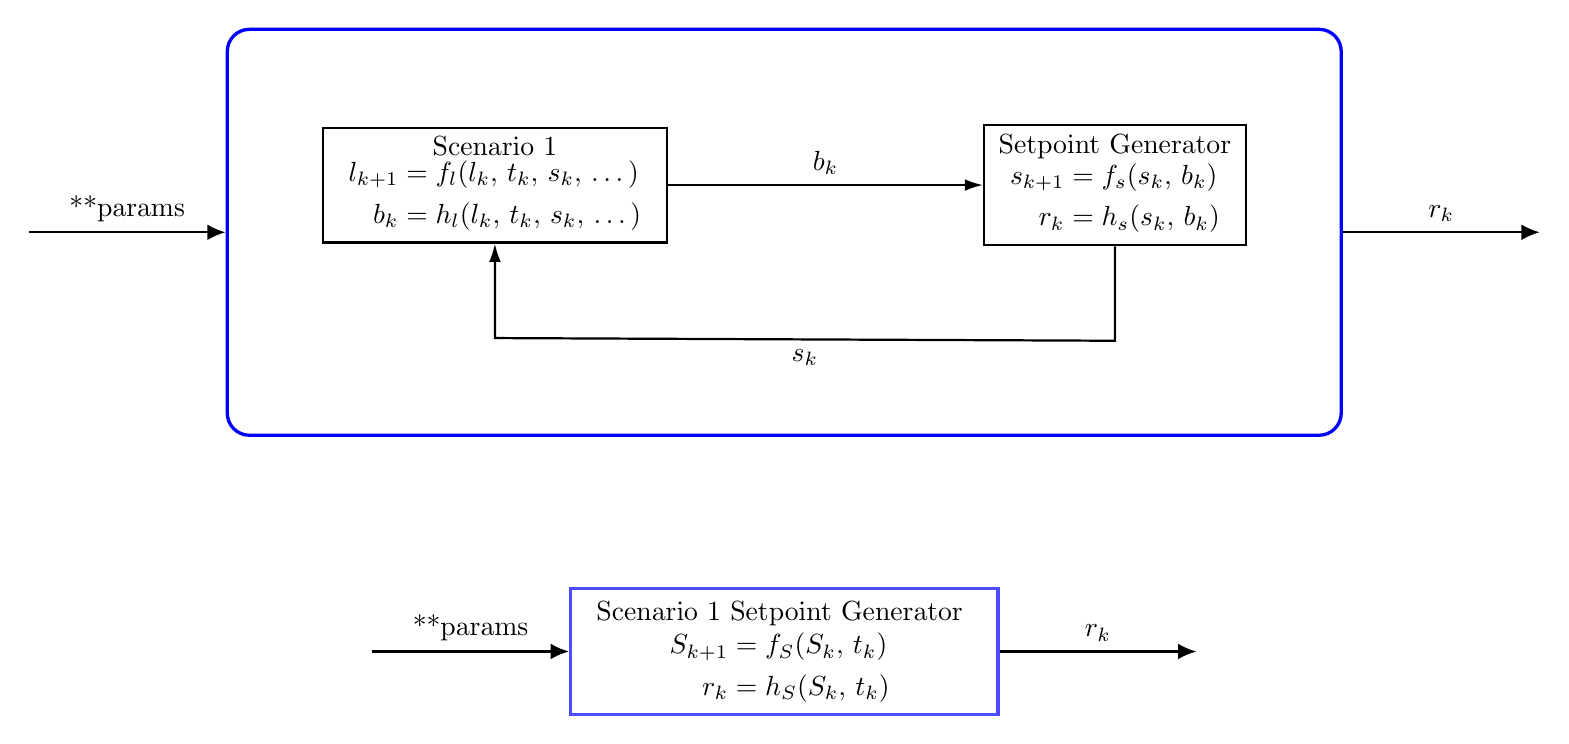
\begin{tikzpicture}[
  block/.style = {
    draw,
    thick,
    minimum height=3em,
    minimum width=7em,
    align=center
  },
  wrapper/.style = {
    draw=blue,
    very thick,
    rounded corners=8pt,
    inner sep=1.2cm
  },
  blueblock/.style = {
    draw=blue!70,
    very thick,
    minimum height=3em,
    minimum width=6em,
    align=center
  },
  arrow/.style = {thick, -{Latex[width=2mm]}},
  internal_arrow/.style = {
    thick,
    draw=black,
    -{Latex[width=1.5mm]}
  },
  node distance=2.5cm and 2.5cm
]

% ======================================================
% TOP SYSTEM (unchanged)
% ======================================================

\node[block] (siggen) {
  Setpoint Generator\\  
  \begin{tabular}{c}
    $\begin{aligned}
      s_{k+1} &= f_s(s_k,\,b_k) \\
      r_k &= h_s(s_k,\,b_k)
    \end{aligned}$
  \end{tabular}
};

\node[block, left=4cm of siggen] (button) {
  Scenario 1\\
  \begin{tabular}{c}
    $\begin{aligned}
      l_{k+1} &= f_l(l_k,\,t_k,\,s_k,\,\dots) \\
      b_k &= h_l(l_k,\,t_k,\,s_k,\,\dots)
    \end{aligned}$
  \end{tabular}
};

\draw[internal_arrow]
  (button.east) -- node[above] {$b_k$} (siggen.west);

\coordinate (sk_down) at ($(siggen.south)+(0,-1.2)$);
\coordinate (sk_left) at ($(button.south)+(0,-1.2)$);

\draw[internal_arrow]
  (siggen.south)
    -- (sk_down)
    -- node[midway,below] {$s_k$} (sk_left)
    -- (button.south);

\begin{scope}[on background layer]
  \node[wrapper, fit=(button)(siggen)(sk_down)] (wrap_top) {};
\end{scope}

\coordinate (external_params_top) at ($(wrap_top.west)+(-2.5,0)$);
\draw[arrow]
  (external_params_top) -- node[above] {**params} (wrap_top.west);

\draw[arrow]
  (wrap_top.east) -- ++(2.5,0) node[midway,above] {$r_k$};

% ======================================================
% BOTTOM SYSTEM: Scenario 1 Setpoint (single blue block)
% ======================================================

\node[blueblock, below=4.5cm of wrap_top.center] (setpoint) {
  \begin{tabular}{c}
    Scenario 1 Setpoint Generator\\
    $\begin{aligned}
      S_{k+1} &= f_S(S_k,\, t_k) \\
      r_k &= h_S(S_k,\,t_k)
    \end{aligned}$
  \end{tabular}
};

% External arrows for bottom system
\coordinate (external_params_bottom) at ($(setpoint.west)+(-2.5,0)$);
\draw[arrow]
  (external_params_bottom) -- node[above] {**params} (setpoint.west);

\draw[arrow]
  (setpoint.east) -- ++(2.5,0) node[midway,above] {$r_k$};

\end{tikzpicture}
\end{document}
